\documentclass[]{book}
\usepackage{lmodern}
\usepackage{amssymb,amsmath}
\usepackage{ifxetex,ifluatex}
\usepackage{fixltx2e} % provides \textsubscript
\ifnum 0\ifxetex 1\fi\ifluatex 1\fi=0 % if pdftex
  \usepackage[T1]{fontenc}
  \usepackage[utf8]{inputenc}
\else % if luatex or xelatex
  \ifxetex
    \usepackage{mathspec}
  \else
    \usepackage{fontspec}
  \fi
  \defaultfontfeatures{Ligatures=TeX,Scale=MatchLowercase}
    \setmonofont[Mapping=tex-ansi,Scale=0.7]{Source Code Pro}
\fi
% use upquote if available, for straight quotes in verbatim environments
\IfFileExists{upquote.sty}{\usepackage{upquote}}{}
% use microtype if available
\IfFileExists{microtype.sty}{%
\usepackage{microtype}
\UseMicrotypeSet[protrusion]{basicmath} % disable protrusion for tt fonts
}{}
\usepackage[margin=1in]{geometry}
\usepackage{hyperref}
\PassOptionsToPackage{usenames,dvipsnames}{color} % color is loaded by hyperref
\hypersetup{unicode=true,
            pdftitle={A solution to ggplot2-book},
            pdfauthor={Raju Rimal},
            colorlinks=true,
            linkcolor=Maroon,
            citecolor=Blue,
            urlcolor=Blue,
            breaklinks=true}
\urlstyle{same}  % don't use monospace font for urls
\usepackage{natbib}
\bibliographystyle{apalike}
\usepackage{color}
\usepackage{fancyvrb}
\newcommand{\VerbBar}{|}
\newcommand{\VERB}{\Verb[commandchars=\\\{\}]}
\DefineVerbatimEnvironment{Highlighting}{Verbatim}{commandchars=\\\{\}}
% Add ',fontsize=\small' for more characters per line
\usepackage{framed}
\definecolor{shadecolor}{RGB}{248,248,248}
\newenvironment{Shaded}{\begin{snugshade}}{\end{snugshade}}
\newcommand{\KeywordTok}[1]{\textcolor[rgb]{0.13,0.29,0.53}{\textbf{#1}}}
\newcommand{\DataTypeTok}[1]{\textcolor[rgb]{0.13,0.29,0.53}{#1}}
\newcommand{\DecValTok}[1]{\textcolor[rgb]{0.00,0.00,0.81}{#1}}
\newcommand{\BaseNTok}[1]{\textcolor[rgb]{0.00,0.00,0.81}{#1}}
\newcommand{\FloatTok}[1]{\textcolor[rgb]{0.00,0.00,0.81}{#1}}
\newcommand{\ConstantTok}[1]{\textcolor[rgb]{0.00,0.00,0.00}{#1}}
\newcommand{\CharTok}[1]{\textcolor[rgb]{0.31,0.60,0.02}{#1}}
\newcommand{\SpecialCharTok}[1]{\textcolor[rgb]{0.00,0.00,0.00}{#1}}
\newcommand{\StringTok}[1]{\textcolor[rgb]{0.31,0.60,0.02}{#1}}
\newcommand{\VerbatimStringTok}[1]{\textcolor[rgb]{0.31,0.60,0.02}{#1}}
\newcommand{\SpecialStringTok}[1]{\textcolor[rgb]{0.31,0.60,0.02}{#1}}
\newcommand{\ImportTok}[1]{#1}
\newcommand{\CommentTok}[1]{\textcolor[rgb]{0.56,0.35,0.01}{\textit{#1}}}
\newcommand{\DocumentationTok}[1]{\textcolor[rgb]{0.56,0.35,0.01}{\textbf{\textit{#1}}}}
\newcommand{\AnnotationTok}[1]{\textcolor[rgb]{0.56,0.35,0.01}{\textbf{\textit{#1}}}}
\newcommand{\CommentVarTok}[1]{\textcolor[rgb]{0.56,0.35,0.01}{\textbf{\textit{#1}}}}
\newcommand{\OtherTok}[1]{\textcolor[rgb]{0.56,0.35,0.01}{#1}}
\newcommand{\FunctionTok}[1]{\textcolor[rgb]{0.00,0.00,0.00}{#1}}
\newcommand{\VariableTok}[1]{\textcolor[rgb]{0.00,0.00,0.00}{#1}}
\newcommand{\ControlFlowTok}[1]{\textcolor[rgb]{0.13,0.29,0.53}{\textbf{#1}}}
\newcommand{\OperatorTok}[1]{\textcolor[rgb]{0.81,0.36,0.00}{\textbf{#1}}}
\newcommand{\BuiltInTok}[1]{#1}
\newcommand{\ExtensionTok}[1]{#1}
\newcommand{\PreprocessorTok}[1]{\textcolor[rgb]{0.56,0.35,0.01}{\textit{#1}}}
\newcommand{\AttributeTok}[1]{\textcolor[rgb]{0.77,0.63,0.00}{#1}}
\newcommand{\RegionMarkerTok}[1]{#1}
\newcommand{\InformationTok}[1]{\textcolor[rgb]{0.56,0.35,0.01}{\textbf{\textit{#1}}}}
\newcommand{\WarningTok}[1]{\textcolor[rgb]{0.56,0.35,0.01}{\textbf{\textit{#1}}}}
\newcommand{\AlertTok}[1]{\textcolor[rgb]{0.94,0.16,0.16}{#1}}
\newcommand{\ErrorTok}[1]{\textcolor[rgb]{0.64,0.00,0.00}{\textbf{#1}}}
\newcommand{\NormalTok}[1]{#1}
\usepackage{longtable,booktabs}
\usepackage{graphicx,grffile}
\makeatletter
\def\maxwidth{\ifdim\Gin@nat@width>\linewidth\linewidth\else\Gin@nat@width\fi}
\def\maxheight{\ifdim\Gin@nat@height>\textheight\textheight\else\Gin@nat@height\fi}
\makeatother
% Scale images if necessary, so that they will not overflow the page
% margins by default, and it is still possible to overwrite the defaults
% using explicit options in \includegraphics[width, height, ...]{}
\setkeys{Gin}{width=\maxwidth,height=\maxheight,keepaspectratio}
\IfFileExists{parskip.sty}{%
\usepackage{parskip}
}{% else
\setlength{\parindent}{0pt}
\setlength{\parskip}{6pt plus 2pt minus 1pt}
}
\setlength{\emergencystretch}{3em}  % prevent overfull lines
\providecommand{\tightlist}{%
  \setlength{\itemsep}{0pt}\setlength{\parskip}{0pt}}
\setcounter{secnumdepth}{5}
% Redefines (sub)paragraphs to behave more like sections
\ifx\paragraph\undefined\else
\let\oldparagraph\paragraph
\renewcommand{\paragraph}[1]{\oldparagraph{#1}\mbox{}}
\fi
\ifx\subparagraph\undefined\else
\let\oldsubparagraph\subparagraph
\renewcommand{\subparagraph}[1]{\oldsubparagraph{#1}\mbox{}}
\fi

%%% Use protect on footnotes to avoid problems with footnotes in titles
\let\rmarkdownfootnote\footnote%
\def\footnote{\protect\rmarkdownfootnote}

%%% Change title format to be more compact
\usepackage{titling}

% Create subtitle command for use in maketitle
\newcommand{\subtitle}[1]{
  \posttitle{
    \begin{center}\large#1\end{center}
    }
}

\setlength{\droptitle}{-2em}
  \title{A solution to ggplot2-book}
  \pretitle{\vspace{\droptitle}\centering\huge}
  \posttitle{\par}
  \author{Raju Rimal}
  \preauthor{\centering\large\emph}
  \postauthor{\par}
  \predate{\centering\large\emph}
  \postdate{\par}
  \date{2017-05-19}

\usepackage{booktabs}
\usepackage{amsthm}
\makeatletter
\def\thm@space@setup{%
  \thm@preskip=8pt plus 2pt minus 4pt
  \thm@postskip=\thm@preskip
}
\makeatother

\begin{document}
\maketitle

{
\hypersetup{linkcolor=black}
\setcounter{tocdepth}{1}
\tableofcontents
}
\chapter*{Prerequisites}\label{prerequisites}
\addcontentsline{toc}{chapter}{Prerequisites}

This is a solution to the problems in ggplot2-book. In order to run all
the solution, following packages need to be installed and loaded.

\begin{Shaded}
\begin{Highlighting}[]
\CommentTok{# devtools::install_github("hadley/tidyverse")}
\NormalTok{pkgs <-}\StringTok{ }\KeywordTok{c}\NormalTok{(}\StringTok{"ggplot2"}\NormalTok{, }\StringTok{"dplyr"}\NormalTok{, }\StringTok{"pander"}\NormalTok{)}
\ControlFlowTok{for}\NormalTok{ (pkg }\ControlFlowTok{in}\NormalTok{ pkgs) }\KeywordTok{require}\NormalTok{(pkg, }\DataTypeTok{character.only =} \OtherTok{TRUE}\NormalTok{)}
\end{Highlighting}
\end{Shaded}

\chapter{Getting Started}\label{getting-started}

\section{Fuel economy data}\label{fuel-economy-data}

\subsection{Exercise 2.2.1}\label{exercise-2.2.1}

\begin{enumerate}
\def\labelenumi{\arabic{enumi}.}
\item
  List five functions that you could use to get more information about
  the \texttt{mpg} dataset. \texttt{str}, \texttt{summary}
\item
  How can you find out what other datasets are included with ggplot2?

\begin{Shaded}
\begin{Highlighting}[]
\NormalTok{data_ggplot <-}\StringTok{ }\KeywordTok{data}\NormalTok{(}\DataTypeTok{package =} \StringTok{"ggplot2"}\NormalTok{)}
\KeywordTok{pander}\NormalTok{(data_ggplot}\OperatorTok{$}\NormalTok{result[, }\OperatorTok{-}\KeywordTok{c}\NormalTok{(}\DecValTok{1}\OperatorTok{:}\DecValTok{2}\NormalTok{)], }\DataTypeTok{justify =} \StringTok{"rl"}\NormalTok{, }
       \DataTypeTok{split.cells =} \DecValTok{50}\NormalTok{, }\DataTypeTok{emphasize.verbatim.cols =} \DecValTok{1}\NormalTok{,}
       \DataTypeTok{caption =} \StringTok{"(}\CharTok{\textbackslash{}\textbackslash{}}\StringTok{#tab:ggplot2-data) Datasets in ggplot2 package"}\NormalTok{)}
\end{Highlighting}
\end{Shaded}

  \begin{longtable}[]{@{}rl@{}}
  \caption{\label{tab:ggplot2-data} Datasets in ggplot2
  package}\tabularnewline
  \toprule
  \begin{minipage}[b]{0.22\columnwidth}\raggedleft\strut
  Item\strut
  \end{minipage} &
  \begin{minipage}[b]{0.61\columnwidth}\raggedright\strut
  Title\strut
  \end{minipage}\tabularnewline
  \midrule
  \endfirsthead
  \toprule
  \begin{minipage}[b]{0.22\columnwidth}\raggedleft\strut
  Item\strut
  \end{minipage} &
  \begin{minipage}[b]{0.61\columnwidth}\raggedright\strut
  Title\strut
  \end{minipage}\tabularnewline
  \midrule
  \endhead
  \begin{minipage}[t]{0.22\columnwidth}\raggedleft\strut
  \texttt{diamonds}\strut
  \end{minipage} &
  \begin{minipage}[t]{0.61\columnwidth}\raggedright\strut
  Prices of 50,000 round cut diamonds\strut
  \end{minipage}\tabularnewline
  \begin{minipage}[t]{0.22\columnwidth}\raggedleft\strut
  \texttt{economics}\strut
  \end{minipage} &
  \begin{minipage}[t]{0.61\columnwidth}\raggedright\strut
  US economic time series\strut
  \end{minipage}\tabularnewline
  \begin{minipage}[t]{0.22\columnwidth}\raggedleft\strut
  \texttt{economics\_long}\strut
  \end{minipage} &
  \begin{minipage}[t]{0.61\columnwidth}\raggedright\strut
  US economic time series\strut
  \end{minipage}\tabularnewline
  \begin{minipage}[t]{0.22\columnwidth}\raggedleft\strut
  \texttt{faithfuld}\strut
  \end{minipage} &
  \begin{minipage}[t]{0.61\columnwidth}\raggedright\strut
  2d density estimate of Old Faithful data\strut
  \end{minipage}\tabularnewline
  \begin{minipage}[t]{0.22\columnwidth}\raggedleft\strut
  \texttt{luv\_colours}\strut
  \end{minipage} &
  \begin{minipage}[t]{0.61\columnwidth}\raggedright\strut
  `colors()' in Luv space\strut
  \end{minipage}\tabularnewline
  \begin{minipage}[t]{0.22\columnwidth}\raggedleft\strut
  \texttt{midwest}\strut
  \end{minipage} &
  \begin{minipage}[t]{0.61\columnwidth}\raggedright\strut
  Midwest demographics\strut
  \end{minipage}\tabularnewline
  \begin{minipage}[t]{0.22\columnwidth}\raggedleft\strut
  \texttt{mpg}\strut
  \end{minipage} &
  \begin{minipage}[t]{0.61\columnwidth}\raggedright\strut
  Fuel economy data from 1999 and 2008 for 38 popular models of
  car\strut
  \end{minipage}\tabularnewline
  \begin{minipage}[t]{0.22\columnwidth}\raggedleft\strut
  \texttt{msleep}\strut
  \end{minipage} &
  \begin{minipage}[t]{0.61\columnwidth}\raggedright\strut
  An updated and expanded version of the mammals sleep dataset\strut
  \end{minipage}\tabularnewline
  \begin{minipage}[t]{0.22\columnwidth}\raggedleft\strut
  \texttt{presidential}\strut
  \end{minipage} &
  \begin{minipage}[t]{0.61\columnwidth}\raggedright\strut
  Terms of 11 presidents from Eisenhower to Obama\strut
  \end{minipage}\tabularnewline
  \begin{minipage}[t]{0.22\columnwidth}\raggedleft\strut
  \texttt{seals}\strut
  \end{minipage} &
  \begin{minipage}[t]{0.61\columnwidth}\raggedright\strut
  Vector field of seal movements\strut
  \end{minipage}\tabularnewline
  \begin{minipage}[t]{0.22\columnwidth}\raggedleft\strut
  \texttt{txhousing}\strut
  \end{minipage} &
  \begin{minipage}[t]{0.61\columnwidth}\raggedright\strut
  Housing sales in TX\strut
  \end{minipage}\tabularnewline
  \bottomrule
  \end{longtable}
\item
  Apart from the US, most countries use fuel consumption (fuel consumed
  over fixed distance) rather than fuel economy (distance travelled with
  fixed amount of fuel). How could you convert \texttt{cty} and
  \texttt{hwy} into the European standard of l/100km?

\begin{Shaded}
\begin{Highlighting}[]
\NormalTok{litre_per_km <-}\StringTok{ }\ControlFlowTok{function}\NormalTok{(mile_per_gallon) \{}
  \KeywordTok{return}\NormalTok{(}\FloatTok{3.78541} \OperatorTok{/}\StringTok{ }\NormalTok{(}\FloatTok{1.60934} \OperatorTok{*}\StringTok{ }\NormalTok{mile_per_gallon))}
\NormalTok{\}}

\NormalTok{mpg_eu <-}\StringTok{ }\NormalTok{mpg }\OperatorTok
\StringTok{  }\KeywordTok{mutate}\NormalTok{(}\DataTypeTok{cty =} \KeywordTok{litre_per_km}\NormalTok{(cty) }\OperatorTok{*}\StringTok{ }\DecValTok{100}\NormalTok{,}
         \DataTypeTok{hwy =} \KeywordTok{litre_per_km}\NormalTok{(hwy) }\OperatorTok{*}\StringTok{ }\DecValTok{100}\NormalTok{)}
\end{Highlighting}
\end{Shaded}
\item
  Which manufacturer has the most the models in this dataset? Which
  model has the most variations? Does your answer change if you remove
  the redundant specification of drive train (e.g. ``pathfinder 4wd'',
  ``a4 quattro'') from the model name?

  \textbf{Manufacturer with Most models:}

\begin{Shaded}
\begin{Highlighting}[]
\NormalTok{mpg }\OperatorTok\StringTok{ }
\StringTok{  }\KeywordTok{group_by}\NormalTok{(manufacturer) }\OperatorTok\StringTok{ }
\StringTok{  }\KeywordTok{summarize}\NormalTok{(}\DataTypeTok{model_count =} \KeywordTok{length}\NormalTok{(}\KeywordTok{unique}\NormalTok{(model))) }\OperatorTok\StringTok{ }
\StringTok{  }\KeywordTok{arrange}\NormalTok{(}\OperatorTok{-}\NormalTok{model_count) }\OperatorTok\StringTok{ }
\StringTok{  }\KeywordTok{ggplot}\NormalTok{(}\KeywordTok{aes}\NormalTok{(model_count, }\KeywordTok{reorder}\NormalTok{(manufacturer, model_count))) }\OperatorTok{+}
\StringTok{  }\KeywordTok{geom_point}\NormalTok{() }\OperatorTok{+}
\StringTok{  }\KeywordTok{labs}\NormalTok{(}\DataTypeTok{x =} \StringTok{"Total Number of unique Models"}\NormalTok{, }\DataTypeTok{y =} \OtherTok{NULL}\NormalTok{)}
\end{Highlighting}
\end{Shaded}

  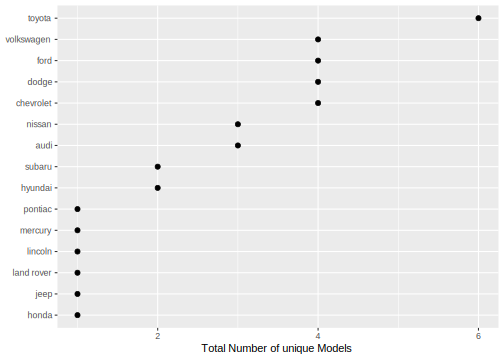
\includegraphics{ggplot2-solution_files/figure-latex/unnamed-chunk-5-1.pdf}

  \textbf{Model with most variations:}

\begin{Shaded}
\begin{Highlighting}[]
\NormalTok{mpg }\OperatorTok\StringTok{ }
\StringTok{  }\KeywordTok{mutate}\NormalTok{(}\DataTypeTok{model_trim =} \KeywordTok{gsub}\NormalTok{(}\StringTok{"([a-zA-Z0-9]+).*"}\NormalTok{, }\StringTok{"}\CharTok{\textbackslash{}\textbackslash{}}\StringTok{1"}\NormalTok{, model)) }\OperatorTok\StringTok{ }
\StringTok{  }\KeywordTok{group_by}\NormalTok{(model) }\OperatorTok\StringTok{ }
\StringTok{  }\KeywordTok{summarize}\NormalTok{(}\DataTypeTok{variation =} \KeywordTok{length}\NormalTok{(model)) }\OperatorTok\StringTok{ }
\StringTok{  }\KeywordTok{arrange}\NormalTok{(}\OperatorTok{-}\NormalTok{variation) }\OperatorTok\StringTok{ }
\StringTok{  }\KeywordTok{ggplot}\NormalTok{(}\KeywordTok{aes}\NormalTok{(variation, }\KeywordTok{reorder}\NormalTok{(model, variation))) }\OperatorTok{+}
\StringTok{  }\KeywordTok{geom_point}\NormalTok{() }\OperatorTok{+}
\StringTok{  }\KeywordTok{labs}\NormalTok{(}\DataTypeTok{x =} \StringTok{"Total number of cars in each model"}\NormalTok{, }\DataTypeTok{y =} \OtherTok{NULL}\NormalTok{)}
\end{Highlighting}
\end{Shaded}

  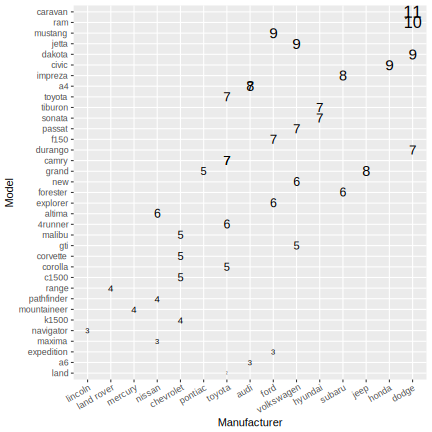
\includegraphics{ggplot2-solution_files/figure-latex/unnamed-chunk-6-1.pdf}

  \textbf{Variation after removing redundant specification:}

\begin{Shaded}
\begin{Highlighting}[]
\NormalTok{mpg }\OperatorTok\StringTok{ }
\StringTok{  }\KeywordTok{mutate}\NormalTok{(}\DataTypeTok{model_trim =} \KeywordTok{gsub}\NormalTok{(}\StringTok{"([a-zA-Z0-9]+).*"}\NormalTok{, }\StringTok{"}\CharTok{\textbackslash{}\textbackslash{}}\StringTok{1"}\NormalTok{, model)) }\OperatorTok\StringTok{ }
\StringTok{  }\KeywordTok{group_by}\NormalTok{(model_trim) }\OperatorTok\StringTok{ }
\StringTok{  }\KeywordTok{summarize}\NormalTok{(}\DataTypeTok{variation =} \KeywordTok{length}\NormalTok{(model)) }\OperatorTok\StringTok{ }
\StringTok{  }\KeywordTok{arrange}\NormalTok{(}\OperatorTok{-}\NormalTok{variation) }\OperatorTok\StringTok{ }
\StringTok{  }\KeywordTok{ggplot}\NormalTok{(}\KeywordTok{aes}\NormalTok{(variation, }\KeywordTok{reorder}\NormalTok{(model_trim, variation))) }\OperatorTok{+}
\StringTok{  }\KeywordTok{geom_point}\NormalTok{() }\OperatorTok{+}
\StringTok{  }\KeywordTok{labs}\NormalTok{(}\DataTypeTok{x =} \StringTok{"Total number of cars in each model"}\NormalTok{, }\DataTypeTok{y =} \OtherTok{NULL}\NormalTok{)}
\end{Highlighting}
\end{Shaded}

  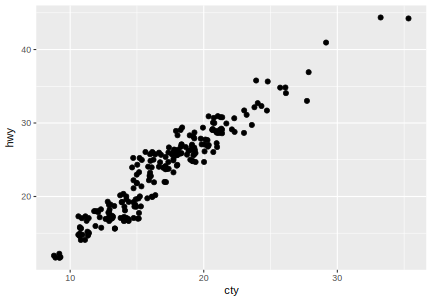
\includegraphics{ggplot2-solution_files/figure-latex/unnamed-chunk-7-1.pdf}
\end{enumerate}

\section{Key components}\label{key-components}

\subsection{Exercises 2.3.1}\label{exercises-2.3.1}

\begin{enumerate}
\def\labelenumi{\arabic{enumi}.}
\item
  How would you describe the relationship between \texttt{cty} and
  \texttt{hwy} ? Do you have any concerns about drawing conclusions from
  that plot?

\begin{Shaded}
\begin{Highlighting}[]
\KeywordTok{ggplot}\NormalTok{(mpg, }\KeywordTok{aes}\NormalTok{(cty, hwy)) }\OperatorTok{+}\StringTok{ }\KeywordTok{geom_point}\NormalTok{(}\DataTypeTok{position =} \StringTok{"jitter"}\NormalTok{)}
\end{Highlighting}
\end{Shaded}

  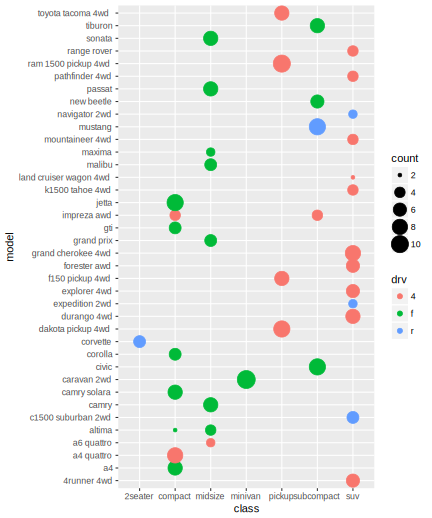
\includegraphics{ggplot2-solution_files/figure-latex/unnamed-chunk-8-1.pdf}
  Its a linear relationship.
\item
  What does
  \texttt{ggplot(mpg,\ aes(model,\ manufacturer))\ +\ geom\ point()}
  show? Is it useful? How could you modify the data to make it more
  informative?

  Not very informative but shows how may models a manufacture have. It
  is more visible if we use \texttt{geom\_count} which uses the
  \texttt{count} summary statistics for each combination of
  \texttt{model} and \texttt{manufacturer}.
\item
  Describe the data, aesthetic mappings and layers used for each of the
  following plots. You'll need to guess a little because you haven't
  seen all the datasets and functions yet, but use your common sense!
  See if you can predict what the plot will look like before running the
  code.

  \begin{enumerate}
  \def\labelenumii{\alph{enumii}.}
  \item
    \texttt{ggplot(mpg,\ aes(cty,\ hwy))\ +\ geom\ point()}

    Data is \texttt{mpg}, \texttt{x} and \texttt{y} axis are mapped to
    \texttt{cty} and \texttt{hwy} variables and a layer of
    \texttt{point} is added.
  \item
    \texttt{ggplot(diamonds,\ aes(carat,\ price))\ +\ geom\ point()}

    Data is \texttt{diamonds}, \texttt{x} and \texttt{y} axis are mapped
    to \texttt{carat} and \texttt{price} variables and a layer of
    \texttt{point} is added.
  \item
    \texttt{ggplot(economics,\ aes(date,\ unemploy))\ +\ geom\ line()}

    Data is \texttt{economics}, \texttt{x} and \texttt{y} axis are
    mapped to \texttt{date} and \texttt{unemploy} variables and a layer
    of \texttt{line} is added.
  \item
    \texttt{ggplot(mpg,\ aes(cty))\ +\ geom\ histogram()}

    Data is \texttt{mpg}, \texttt{x} axis are mapped to \texttt{cty} and
    a layer of \texttt{histogram} is added which uses the default bins
    of \texttt{30}.
  \end{enumerate}
\end{enumerate}

\section{Colour, size, shape and other aesthetic
attributes}\label{colour-size-shape-and-other-aesthetic-attributes}

\subsection{Exercises 2.4.1}\label{exercises-2.4.1}

\begin{enumerate}
\def\labelenumi{\arabic{enumi}.}
\item
  Experiment with the colour, shape and size aesthetics. What happens
  when you map them to continuous values? What about categorical values?
  What happens when you use more than one aesthetic in a plot?
\item
  What happens if you map a continuous variable to shape? Why? What
  happens if you map trans to shape? Why?
\item
  How is drive train related to fuel economy? How is drive train related
  to engine size and class?

\begin{Shaded}
\begin{Highlighting}[]
\NormalTok{mpg }\OperatorTok\StringTok{ }
\StringTok{  }\KeywordTok{group_by}\NormalTok{(model, class, drv) }\OperatorTok\StringTok{ }
\StringTok{  }\KeywordTok{summarize}\NormalTok{(}\DataTypeTok{count =} \KeywordTok{n}\NormalTok{()) }\OperatorTok\StringTok{ }
\StringTok{  }\KeywordTok{ggplot}\NormalTok{(}\KeywordTok{aes}\NormalTok{(class, model, }\DataTypeTok{color =}\NormalTok{ drv, }\DataTypeTok{size =}\NormalTok{ count)) }\OperatorTok{+}\StringTok{ }
\StringTok{  }\KeywordTok{geom_point}\NormalTok{()}
\end{Highlighting}
\end{Shaded}

  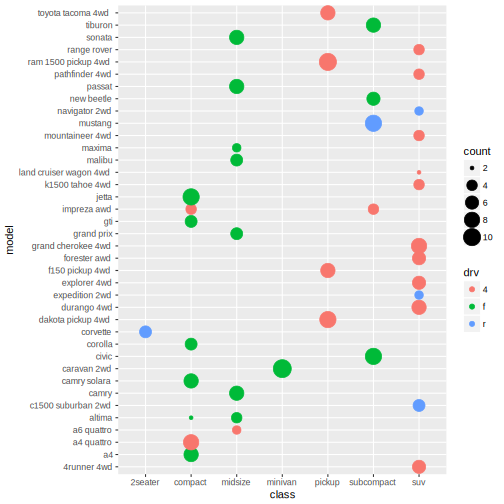
\includegraphics{ggplot2-solution_files/figure-latex/unnamed-chunk-9-1.pdf}

  Here, we see that \texttt{suv} and \texttt{pickup} has mostly 4 whell
  drive while rest are front-wheeled drive.
\end{enumerate}

\section{Facetting}\label{facetting}

\subsection{Exercises 2.5.1}\label{exercises-2.5.1}

\begin{enumerate}
\def\labelenumi{\arabic{enumi}.}
\item
  What happens if you try to facet by a continuous variable like
  \texttt{hwy} ? What about \texttt{cyl} ? What's the key difference?

  When a continuous variables, like \texttt{hwy}, is used for facet,
  ggplot converts it into factor and creates facet from all unique value
  of that continuous variable. Here \texttt{hwy} has many unique values
  so we will get many facets for each of them while \texttt{cyl} has few
  discrete values and is useful to use for faceting.
\item
  Use facetting to explore the 3-way relationship between fuel economy,
  engine size, and number of cylinders. How does facetting by number of
  cylinders change your assessement of the relationship between engine
  size and fuel economy?

\begin{Shaded}
\begin{Highlighting}[]
\KeywordTok{ggplot}\NormalTok{(mpg, }\KeywordTok{aes}\NormalTok{(cty, hwy, }\DataTypeTok{color =}\NormalTok{ displ)) }\OperatorTok{+}\StringTok{ }
\StringTok{  }\KeywordTok{geom_point}\NormalTok{(}\DataTypeTok{alpha =} \FloatTok{0.5}\NormalTok{, }\DataTypeTok{position =} \StringTok{"jitter"}\NormalTok{) }\OperatorTok{+}
\StringTok{  }\KeywordTok{facet_grid}\NormalTok{(.}\OperatorTok{~}\NormalTok{cyl, }\DataTypeTok{labeller =}\NormalTok{ label_both)}
\end{Highlighting}
\end{Shaded}

  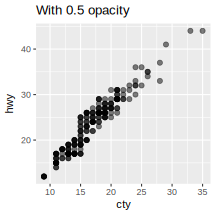
\includegraphics{ggplot2-solution_files/figure-latex/unnamed-chunk-10-1.pdf}

  Here we can see that larger engine size has lower milage in both city
  and highway. In addition, vechile with large number of cylender has
  larger engine size. Further there are very few vechile having 5
  cylinder.
\item
  Read the documentation for \texttt{facet\ wrap()}. What arguments can
  you use to control how many rows and columns appear in the output?

  The \texttt{nrow} and \texttt{ncol} arguments in
  \texttt{facet\_wrap()} controls the number of rows and columns.
\item
  What does the scales argument to facet wrap() do? When might you use
  it?

  Here \texttt{scales} can take three values -- \texttt{free},
  \texttt{free\_x} and \texttt{free\_y}. \texttt{free\_x} gives separate
  x-axis for each facet, \texttt{free\_y} gives separate y-axis for each
  facet and similarly, \texttt{free} gives separate x and y axis for
  each facet.
\end{enumerate}

\bibliography{packages.bib,book.bib}


\end{document}
